\chapter{OTFVis: MATSim's Open-Source Visualizer}
\label{ch:otfvis}
% ##################################################################################################################

\hfill \textbf{Author:} David Strippgen

\begin{center} 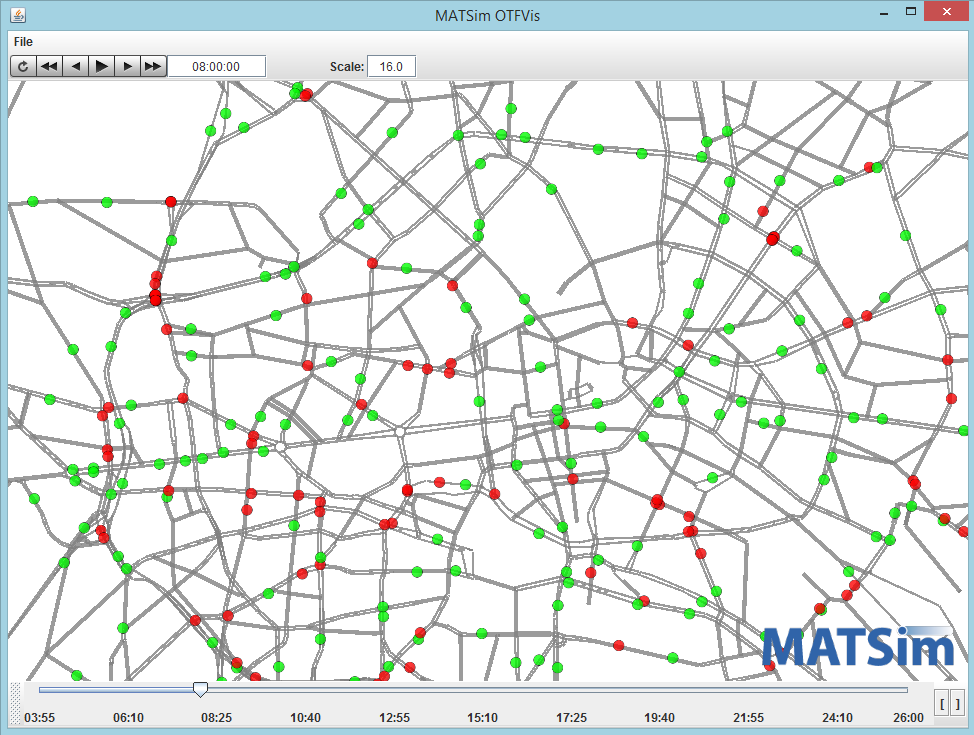
\includegraphics[width=0.4\textwidth, angle=0]{extending/figures/otfvis/image06.png} \end{center}

\editdone{This text has undergone the professional edit. Please no grammatical changes anymore! They are most-probably wrong.}

\createStandardInformation{otfvis}{\lstinline{OTFVis} class, \lstinline{RunOTFVis} class}{otfvis}{\citet[][]{Strippgen_PhDThesis_2009}}

% ##################################################################################################################
\section{Introduction}
For most \gls{matsim} users, Via's (Chapter~\ref{ch:via}) free branch will be a good solution for their visualization needs. However, if project demand reaches beyond the given (and fixed) abilities of the Via free version, there is another---though not as stylish---option for \gls{matsim} output visualization, the \gls{otfvis}. 

The short term for ``On the Fly Visualizer'', \gls{otfvis} was designed to support actual visualization of live simulation runs with \gls{matsim}. Therefore, one purpose of the \gls{otfvis} is the debugging of \gls{matsim} (input) data. Nonetheless, playing prerecorded movie (\gls{mvi}) files created from \gls{matsim} events is another way to use \gls{otfvis}. Generally speaking, \gls{otfvis} serves as an open-source counterpart to the possibilities Via gives the \gls{matsim} community. The \gls{otfvis} is written in \gls{java} and available as source code to extend for different \gls{matsim} projects' special needs. Hence, it is possible and desirable to actually extend the \gls{otfvis} functionality, incorporating the user's own data sets and visualizations.

% ################################################################################################################
\section{Using OTFVis} 
In this chapter, we show how to achieve simple things, like creating \gls{mvi}-files from \gls{matsim} run events, how to play these \gls{mvi}-files and how to use a \gls{matsim} \gls{configfile} to view/play an actual simulation with all data (\eg agent's plans) attached. With the latter, it it also possible to examine the data ``on the fly'' by sending queries into the \gls{mobsim} and visualizing the results.

% ============================================================================================
\subsection{MVI Files}
\gls{mvi} files can be generated through the \gls{otfvis}. Under the hood, these files consist of a few binary dumps of \gls{otfvis} data packed into a zip-file. This binary data is created by \gls{java}'s own serialization capabilities. Unfortunately, this setup is not very change-resistant, making it advisable to regard \gls{mvi} files as temporary cached versions of your event files. These \gls{mvi} files can be re-created at any time from the event files. Still, as converting one into the other is a time-prone process, the \gls{mvi} files are a handy tool for temporary storage and fast loading of your visualizations.

% ============================================================================================
\subsection{Starting OTFVis}
\gls{otfvis} is a \gls{matsim} \gls{contribution}. 
There is no actual stable release of the \gls{otfvis} package; 
so, to acquire a working version, a ``nightly build'' needs to be downloaded as shown in Section~\ref{sec:releases-builds}. 
There, one finds the latest \lstinline|otfvis-version-SNAPSHOT-build.zip| file available for download. 
Unzip it to the place where the \lstinline|matsim.jar| already resides; don't forget to extract the \lstinline|libs|-directories found in the respective zip files. 

\gls{otfvis} demands substantial \gls{ram} (depending on your simulation size/\gls{mvi} file); to successfully launch the visualizer, a command line like 
\begin{lstlisting}
java -Xmx500m -cp MATSim-XXX.jar:otfvis/otfvis-XXX.jar org.MATSim.contrib.otfvis.OTFVis
\end{lstlisting}
(exchange ``;'' with ``:'' depending on the used \gls{os})
is a good starting point. 
This will open the dialog window shown in Figure~\ref{fig:otfvis_dialog}, asking for one choice from four possible usages of \gls{otfvis}; 
these will be explained in the next section.

%---------------------------------------------------------------------
\createfigure%
{\gls{otfvis} Start Dialog}%
{\gls{otfvis} Start Dialog}%
{\label{fig:otfvis_dialog}}%
{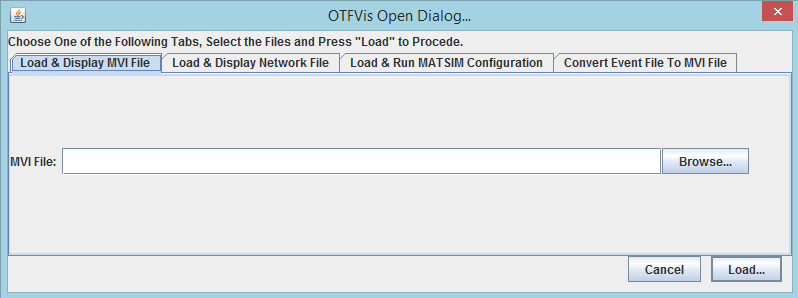
\includegraphics[width=0.95\textwidth, angle=0]{extending/figures/otfvis/image03.png}}%
{}
%---------------------------------------------------------------------

% ============================================================================================
\subsection{Use Cases of OTFVis}
With the open dialog appearing after starting the vanilla \lstinline|OTVFis| class, the following options appear, as shown in Figure~\ref{fig:otfvis_dialog}.
%
\begin{enumerate}\styleEnumerate
	\item Opening a prerecorded \gls{mvi} file,
	\item Opening a network file (for inspection),
	\item Opening a live run of a \gls{matsim} \gls{configfile} (rather memory intensive) or
	\item Converting an event file (plus a given network file) to a movie (\gls{mvi}) file.
\end{enumerate}

Each tab stands for an individual usage. To start a visualization, one chooses the appropriate tab, fills in the necessary data and finally proceeds by pressing the \lstinline|Load...| button located in the bottom left corner of the window.

The next sections provide an overview of different ways to use \gls{otfvis}.

% ---------------------------------------------------------
\subsubsection{Converting Event Files}
Though the first option tab is the most used choice for \gls{otfvis}, the fourth, and last, option tab is a good starting point for exploring the visualizer; after having successfully run a \gls{matsim} simulation, there will typically be some event files at one's disposal. With any of these event files and a given (matching) network file, a \gls{mvi} file can be created. 
Four items: event, network and movie file names, as well as a time period, must be specified for this tab to execute. 
The last parameter is a time period, after which a new sample of the \gls{mobsim}'s state is taken. 
This \gls{mvi}-generation process might be time consuming. For smaller projects, it might be an option to display the outcome in the visualizer right away (by checking the box \lstinline|Open mvi afterwards|). 
If the choice is to just convert the events to a \gls{mvi} file, this can be opened with the first option tab of the visualizer's start dialog at any time. 

From the shell, this process can be started by giving the event file, network file and, optionally, the conversion period as input parameters.

% ---------------------------------------------------------
\subsubsection{Network File Loading}
The second option tab offers the opportunity to examine a network file (\eg for errors). 
It will show a rendering of the given network and also, if so chosen in the preferences, the associated network link IDs for each link. 
This option might be helpful for debugging a freshly converted network, or inspecting specific regions and connections. Loading and interacting with a network file should be very fast. 

The network file can also be given as the sole parameter to \gls{otfvis} with the shell command.

% ---------------------------------------------------------
\subsubsection{Running a MATSim Configuration}
The third, and most advanced, option for running \gls{otfvis} is an actual, live running \gls{mobsim}, visualized in real time (actually much faster than real time; who has all day to watch tiny cars drive around?). This option includes the possibility of exploring the data set and issuing queries into the executing \gls{mobsim}. These queries can display an agent's day plan, show all links driven by agent's crossing a particular link of interest, search for a particular link or node by ID, or answer any user-defined queries. We will see later in this chapter how to program a user's own queries, but for the rest of this section we will detail \gls{otfvis} ``offline'' behavior. 

It is also feasible to input the \gls{configfile} as a single parameter to \gls{otfvis} by starting it from the shell. \gls{otfvis} will make an educated guess whether the input is a config or a network file.

% ---------------------------------------------------------
\subsubsection{Loading \& Displaying an MVI File}
If the first and default option tab is chosen, a \gls{mvi} file is selected and shown as detailed in next section~\ref{sec:otfvis-viewing-an-mvi-file}. This is the most common use case for \gls{otfvis}; the same results can be achieved by starting \gls{otfvis} from the shell with an \gls{mvi} file as an argument.

% ============================================================================================
\subsection{Viewing an MVI File}
\label{sec:otfvis-viewing-an-mvi-file}
An example is illustrated in Figure~\ref{fig:OTFVisRunning}. On the top left of the application, one finds buttons for controlling the file playback. A short summary of the functionality is given in Table~\ref{tab:otfvis-buttonbar}.

This buttonbar is followed by a text field where the desired time can be written for an instant jump. In an \gls{mvi} file, one can jump forward and backward in time, whereas in the live simulation case, going back in time is omitted.

Another way of iterating through the animation is to grab the time slider at the bottom of the application and drag it. 
Opening and closing bracket symbols are located on the left side of the slider; 
by clicking them, one can set the start, or end, time of a time loop to the actual time step given, making 
it possible to restrict playback to a certain space of time.

%---------------------------------------------------------------------
\createfigure%
{Displaying an MVI file}%
{Displaying an MVI file}%
{\label{fig:OTFVisRunning}}%
{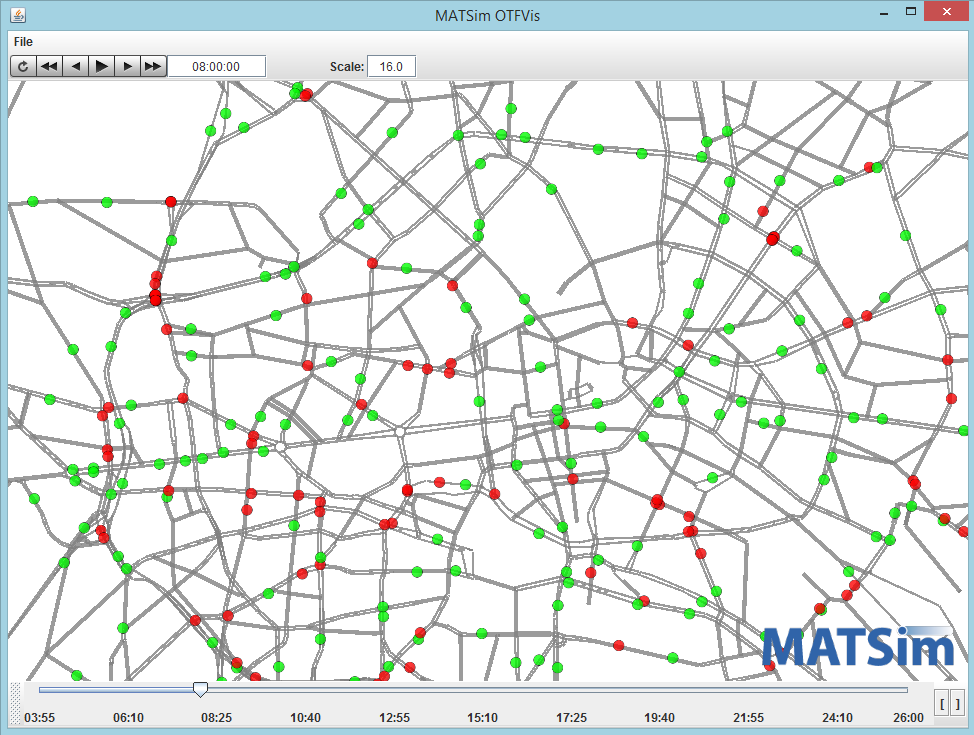
\includegraphics[width=0.95\textwidth, angle=0]{extending/figures/otfvis/image06.png}}%
{}
%---------------------------------------------------------------------
%---------------------------------------------------------------------
\createtable%
{OTFVis Buttonbar}%
{OTFVis Buttonbar}%
{\label{tab:otfvis-buttonbar}}%
{%
  \begin{tabular}[c]{|m{1cm}|m{6cm}|}
    \hline
    \textbf{Icon}  & \textbf{Function} \\
    \hline
		\raisebox{-.17\height}{
\includegraphics[width=0.03\textwidth]{extending/figures/otfvis/image00.png}} & Reset - set time to the start time\\
		\hline
		\raisebox{-.17\height}{
\includegraphics[width=0.03\textwidth]{extending/figures/otfvis/image01.png}} & Large step back\\
		\hline
		\raisebox{-.17\height}{
\includegraphics[width=0.03\textwidth]{extending/figures/otfvis/image09.png}} & Small step back\\
		\hline
		\raisebox{-.17\height}{
\includegraphics[width=0.03\textwidth]{extending/figures/otfvis/image05.png}} & Play \\
		\hline
		\raisebox{-.17\height}{
\includegraphics[width=0.03\textwidth]{extending/figures/otfvis/image07.png}} & Pause \\
		\hline
		\raisebox{-.17\height}{
\includegraphics[width=0.03\textwidth]{extending/figures/otfvis/image02.png}} & Small step forward \\
		\hline
		\raisebox{-.17\height}{
\includegraphics[width=0.03\textwidth]{extending/figures/otfvis/image10.png}} & Large step forward \\
		\hline
  \end{tabular}
}%
{}
%---------------------------------------------------------------------

% ============================================================================================
\subsection{General Interaction with the Main Screen}
Regardless which option for loading data was chosen, interaction with the main display area is the same.
%
\begin{description}\styleDescription
\item[Right button drag:] Extend a rectangle for zooming into the view. Releasing the button will execute a zoom, so the chosen rectangle will best fit the screen.
\item[Middle-Mouse-drag:] Pan (translate) the screen.
\item[Right-Mouse-Click:] Show a context menu (for now only with the option to save the view settings)
\end{description}

% ============================================================================================
\subsection{User Interaction in the Live Mobsim}
When started as a live simulation, \gls{otfvis} will look different than Figure~\ref{fig:OTFVisLive}. 
First, the controls of the simulation's view flow are a restricted subset of those used in \gls{mvi} playback. 
There is no way to reset or rewind the simulation. 
One can still take small or large steps forward. 
A new option is given by the \lstinline|synch| checkbox, which 
determines whether the \gls{mobsim} will stop for each frame the \gls{otfvis} renders, or run independently. 
Usually the \lstinline|un-synched| version will proceed faster, as the \gls{otfvis} output is restricted to a default of about 30\,frames/updates per second and a small \gls{mobsim}'s simulation speed will be a magnitude higher. 
The time-consuming generation of visualization data will also only be necessary for a small fraction of the simulation. 
Length of \gls{otfvis} pauses between frames can be configured in the preferences dialog.

Apart from the reduced control set, there is another UI element new to this \gls{otfvis} option. 
At the bottom of the screen, the scrubbar/time line element is replaced by a ``query'' bar. 
It is possible to code ``queries'' into the \gls{mobsim}, answering questions about its inner state. 
As the simulation is actually happening, all information necessary to run it is available for output. 
This is a clear superset of information available in the event files and in the \gls{mvi} files. 
This rich information infrastructure can be queried and visualized in many ways. 
In the next session, a query example is given.

%---------------------------------------------------------------------
\createfigure%
{Live mode}%
{Live mode}%
{\label{fig:OTFVisLive}}%
{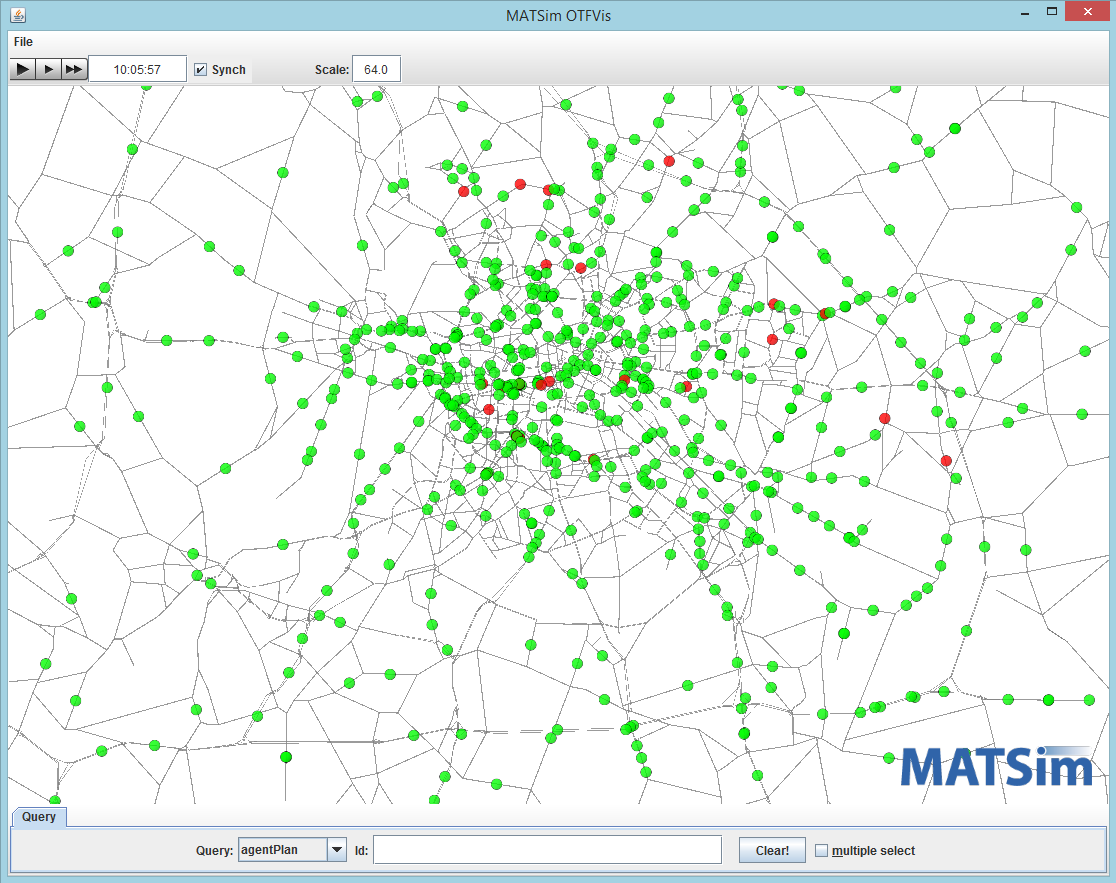
\includegraphics[width=0.95\textwidth, angle=0]{extending/figures/otfvis/image04.png}}%
{}
%---------------------------------------------------------------------

% ============================================================================================
\subsection{Running a Query in OTFVis Real Time Data}
From the dropdown box, one can choose the different query types. 
Often, additional input is necessary, either in the text field next to it or, more often, by clicking into the network. 
To give an example with \lstinline|agent query| selected, a click onto any agent's symbol will give a visualization of this particular agent's day plan. 
This is shown in Figure~\ref{fig:OTFVisAgent}. There are other pre-defined queries. 
These queries are rather project-oriented, so defining own queries will probably be necessary to make best use of this option. 
In the second part of this chapter, we will look into defining own queries.

%---------------------------------------------------------------------
\createfigure%
{Queries}%
{Queries}%
{\label{fig:OTFVisAgent}}%
{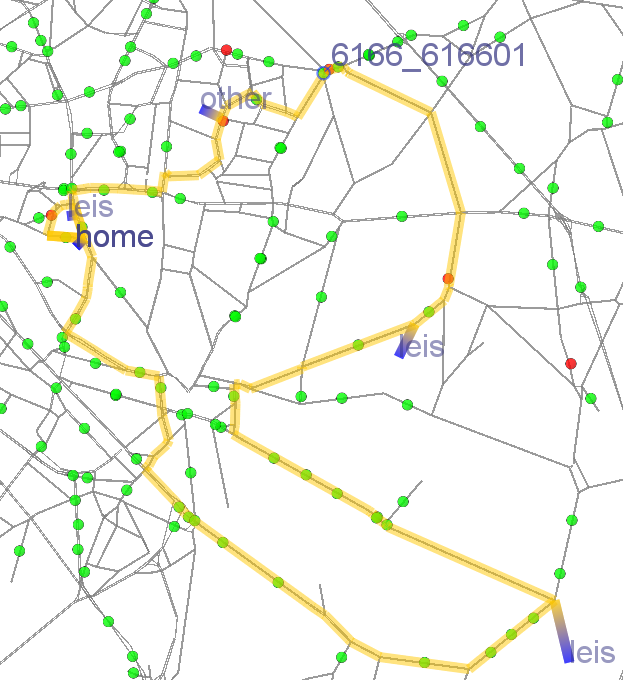
\includegraphics[width=0.35\textwidth, angle=0]{extending/figures/otfvis/image08.png}}%
{}
%---------------------------------------------------------------------

% ##################################################################################################################
\section{Extending OTFVis}
Because it is open source, the \gls{otfvis} is a good starting point for customizing mobsim run visualizations. 
\gls{otfvis} has been written in \gls{java}, but depends heavily on the \gls{jogl} \gls{java} library.% (link). 
\gls{jogl} is a very thin layer within the \gls{os} hardware driver, meaning it will have \gls{os}-specific, native dependencies. 
These should be attended to by the maven-dependency management, but should still be kept in mind when developing for \gls{otfvis}. 
The displaying parts of \gls{otfvis} are based on \gls{opengl}. 
Therefore, it will be necessary to understand \gls{opengl} to create new ways of displaying data. 
In the following sections, we examine how data is computed inside the \gls{otfvis} and how this can be extended.

% ============================================================================================
\subsection{Design Principles of \gls{otfvis}}
The overall goal of \gls{otfvis} design was to have an easy-to-extend, fast visualizer capable of handling huge amounts of data. 
The specific design goals for the visualizer were:
%
\begin{itemize}
\item Abstract data source (data collection) from data display (visualization)
\item Easy extension with own data types
\item Capability for local simulation run on desktop computer
\item Reduction of sent data to a minimum
\item Visualization that connects to running simulation (on-the-fly)
\item Minimally-invasive format for existing \gls{matsim} code
\item Enough speed for large scenarios
\item Visualization that reads from post-mortem dump (\gls{mvi} file)
\item Use hardware support for drawing
\end{itemize}
%
\gls{matsim} runs can easily engage millions of agents traveling a network. To make a visualization of these large data sets feasible, two measures have been taken. A quad tree structure was implemented to ensure that only the smallest set of data necessary to display the visible sector of the network is transferred. The quad tree is a simple data structure to aggregate spatial data and retrieve parts of it efficiently for real time visualization. Apart from data structures, hardware is also used to speed up displaying the simulation. \gls{opengl} is a platform-independent \gls{api} for interfacing graphics hardware, specifically the 3D acceleration chips implemented in every contemporary computer. With the aid of 3D graphics hardware, millions of agents can be displayed in real time. Other measures were taken to segregate data extraction from data visualization, like the reader/writer pairs presented in the next section.

% ============================================================================================
\subsection{Readers and Writers}
\gls{otfvis} was designed to be minimally dependent on the \gls{mobsim} used. Data formats applied within the \gls{mobsim} should be abstracted from data used in \gls{otfvis}, meaning that any data passed to the visualizer will have to run through some stages of abstraction.

The first stage is a writer-reader pair, responsible for transferring a certain set of data to the \gls{otfvis}. The writer will understand the data format of the hosting \gls{mobsim} and convert it to simple data types, like float or string values. A set of these writers, all using a joint byte buffer to aggregate the data, will be called after each \gls{mobsim} step to accumulate data. This array of bytes is then sent to the visualizer, which, in the original design, could be run anywhere in your network.

For each writer, there has to be a sibling-reader class, responsible for reading back extracted data from the byte buffer. 
It is crucial to ensure that these pairs work synchronously. Most Writer/Reader-pairs are implemented in the same class, since having the source-code at the same place reduces errors in the synchronization.

Apparently, it can be necessary, or at least useful, to have different ways of visualizing data on the \gls{otfvis} front-end. Thus, actual readers are not responsible for the drawing of a certain data set. A third kind of class is responsible for that, the drawer classes.

% ============================================================================================
\subsection{Visualization of the Data}
The reader objects in the quad tree will generate separate drawer objects for displaying ``their'' information and add these to another data structure, called \lstinline|SceneGraph|, which is responsible for the actual drawing onto an \gls{opengl} canvas. 
Displaying data in an interactive application will make re-draws of the display necessary for a variety of reasons: displaying menus, animations, zooming, panning and other user interactions. 
Not all of these changes introduce new data from the \gls{mobsim}. 
Zooming into the network will not imply reading data from the \gls{mobsim}; panning the view most certainly will. 
When no new data is needed, the scene graph is capable to handle all operations, no reader/writer class will be accessed and displaying is solely done with existing drawers. 
On the other hand, if new data is demanded, the scene graph will be ``invalidated'' (a term lent from the \gls{opengl} community); thus, the graph will be dismissed and all relevant readers will be asked for new drawer objects representing the actual view. The scene graph is mainly a list of drawer objects; as an extra structuring unit, these drawers can be sent into different layers, to render them more effective.

% ============================================================================================
\subsection{Layers}
To make sure that only data actually necessary for drawing the particular area visible in the viewport is sent, writers should minimize the data packets, so the quad tree can make a spatial data reduction. This seems somewhat in opposition to \gls{opengl} or any graphics \gls{api}). The \gls{api} wants maximal data to be accumulated, to optimize output through the underlying hardware graphics pipeline. 
Think of an assembly line vs. a handcrafted item; whenever the flow of data is interrupted, the assembly line stalls and graphics performance derogates. 
To ease this issue, ``layers'' have been introduced to \gls{otfvis}. 
Any drawer (responsible for a bit of information) can be assigned to a layer and 
these layers will ultimately be summoned to draw the screen's content. 
It is up to the layer to optimize the execution of the drawers when necessary. 
For example, a network layer might store all network info from the drawer in one array, or display a list to optimize drawing of the network; (often in \gls{opengl}, it is advisable to rather let the hardware decide what to draw. 
%\Karen{please check this last half-sentence to make sure I got the meaning right... Thanks!} \ah{correct}
It might be faster to have all complete data residing in graphics hardware memory, rather than to transfer the reduced information set every frame). There are three layers predefined in \gls{otfvis}. 
The \lstinline|networkLayer| contains the static street net, the \lstinline|agentLayer| the actual dynamic agents and a third layer, the \lstinline|miscellaneousLayer|,  contains additional data.

% ============================================================================================
\subsection{Patching the Connections}
In total, there are four basic elements involved in the visualization: writers, readers, drawers and layers. 
An additional class configures how the first two work together: \lstinline|OTFConnectionManager|.

This class maps several routes for the information coming from the \gls{mobsim}, building a chain of responsibility. 
Each data item starts at a link in our network. 
An \lstinline|OTFDataWriter| object is responsible for extracting the desired data from the link and writing it into a \lstinline|ByteBuffer|. 
Complementing this, an associated \lstinline|OTFDataReader| is needed to retrieve data from the buffer. 
This item will also be responsible for adding a drawable item derived from the class \lstinline|OTFGLAbstractDrawable| to the scene graph representing the actual screen content. 
The connection between these items is made by adding entries into the \lstinline|OTFConnectionManager|, with calls to \lstinline|OTFConnectionManager.connectLinkToWriter(OTFDataWriter)| 
and \lstinline|OTFConnectionManager.connectLinkToWriter(OTFDataWriter, OTFDataReader)|, respectively.
 
Example (from the \lstinline|OTFClientLive.java|):

\lstinline|conMan.connectLinkToWriter(OTFLinkAgentsHandler.Writer.class);| \\
\lstinline|conMan.connectWriterToReader(OTFLinkAgentsHandler.Writer.class,|
\lstinline|OTFLinkAgentsHandler.class);|

% ============================================================================================
\subsection{Sending the Data}
The class \lstinline|OTFLinkAgentsHandler| should give a good example of extracting, sending, receiving and displaying data in the \gls{otfvis} context. The method \lstinline|invalidate| is called whenever the actual scene graph has been dismissed and needs to be rebuilt. 
In this case, a valid representation of the object's state should be added to the new scene graph. 
This also means that for drawing the actual scene, no additional reading will take place, unless 
there is a change in the visible data: then, this update is triggered.

% ============================================================================================
\subsection{Performance Considerations}
When implementing new ways to visualize data, the following guidelines should be kept in mind.

If the data is spatially distributed over the whole network and is updated frequently, an \lstinline|OTFDataWriter/Reader| pair should be considered. 
It will reduce data updating to times when the data is actually visible, not creating, transporting or drawing the data otherwise. If a fraction of the data needs to be transferred only once---because it is static over the time of the simulation---it can be sent with the \lstinline|writeConstData()| method; otherwise using \lstinline|writeDynData()| is advised. 
If the data is sparse and little information is transmitted or it has no discernible spatial cohesion, it might be simpler to just add it to the server quad tree as additional data with a call to \lstinline|OTFServerQuadTree.addAdditionalElement()|. 

% ============================================================================================
\subsection{Sending Live Data}
Flow of data within \gls{otfvis} is almost always a one way affair, 
except for one important issue: sending queries into the simulation. In case of a live simulation run, visualized with help from the \lstinline|OTFVisLiveClient| class, queries can be sent into the simulation. 
Again, the methods involved in this process are threefold; queries will be realized through an object derived from the abstract class \lstinline|AbstractQuery|. Such an object initiates several methods that will be used as callback over the lifetime of the query.

First, a new query is sent to the server and the method \lstinline|installQuery()| is called. 
In this method, all relevant parts (network, population, events) of the simulation run can be accessed and data can be collected. 
The visualizer framework will later repeatedly call the \lstinline|result()| method, to retrieve an \lstinline|OTFQueryResult| object. 
This has to implement a \lstinline|draw()| method, to visualize the results in the given screen context. 
If the result indicates \lstinline|isAlive()|, the \lstinline|query()| method of the \lstinline|AbstractQuery|-derived object will be called with each frame; otherwise, only once.

% ##################################################################################################################








